Prompt Patterns are specific command or instruction formulation strategies or approaches used to interact with the \ac{LLM}. They play a crucial role in eliciting desired and relevant responses from \ac{LLM}, allowing users to communicate their intentions effectively.

Integrating Prompt Patterns with \ac{LLM} involves creating instructions or queries adapted to the context of the task or question you want to address. This is done by taking into account the structure and capabilities of the language model. Figure \ref{prompt-pattern-overview} shows an overview of the interaction between the user, prompt pattern, AI Assisted tools, and \ac{LLM}.

\begin{figure}[!ht]
    \centering
    \caption{\centering Interaction between the User, Prompt Pattern, AI Assisted tools, and
LLM.}\label{prompt-pattern-overview}
    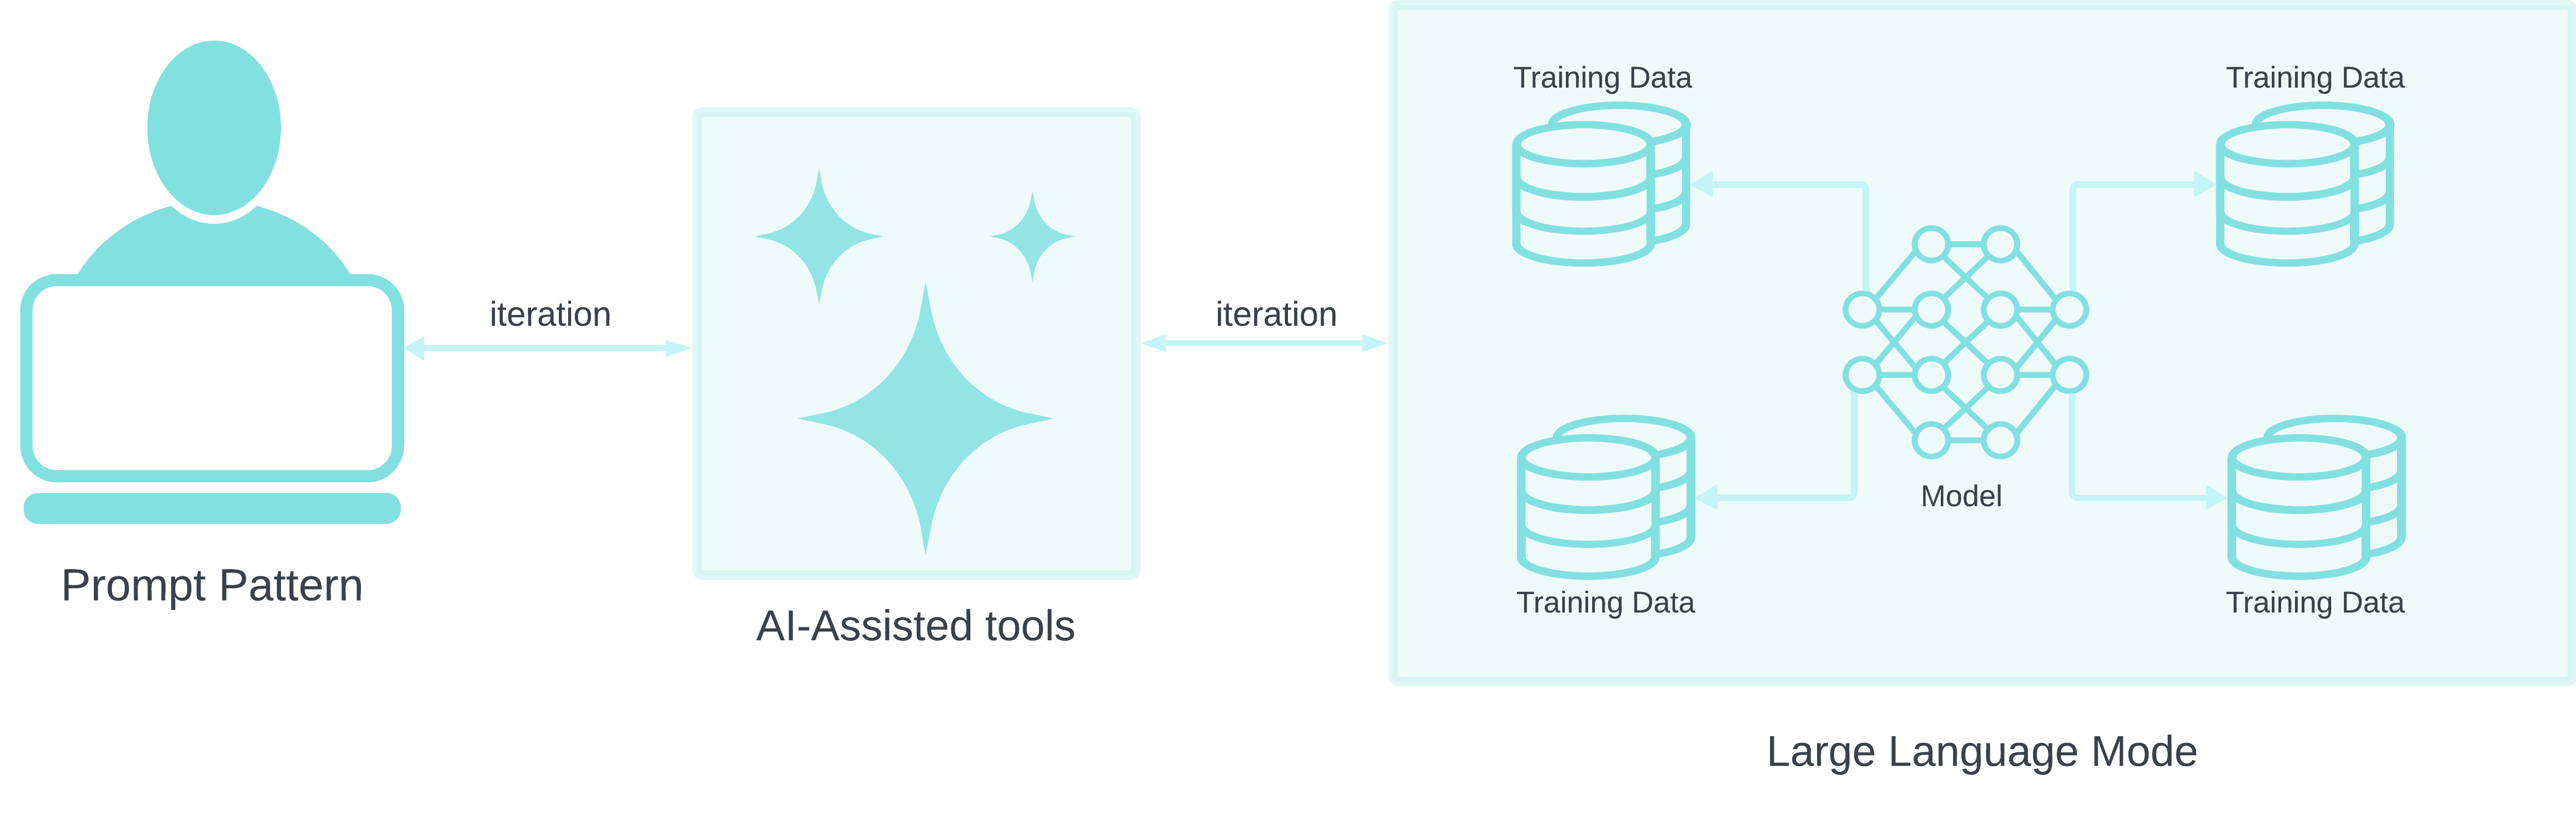
\includegraphics[width=0.95\textwidth]{figures/prompt-patterns-overview.png}
     \objectsource{\objectsourceauthor}
\end{figure}

Successful integration of Prompt Patterns with \ac{LLM} depends on careful wording of commands, considering context sensitivity and keyword choice. It is essential to test and iterate prompt patterns to get the best results, as different \ac{LLM} templates may behave slightly differently.

Chapter introduction
% Ligação com o que veio antes
% Objetivo do capítulo no contexto da tese
% Conteúdo do capítulo

\section{Approach General Description}

Objetivo: usar ferramentas para auxiliary em decisões arquiteturais. 

Do que se trata: se base nos prompt patterns existence. Utiliza padrões existentes, expecializa alguns desses padrões e propõe novos.


Os seguintes padrões existences são usados nesse trabalho:

- \texttt{Padrão 1}: ...
- Padrão 2: ...

* Usar o format de "patlet": (1 frase contexto) (1 frase problema) (1 frase solução)

Os seguintes padrões são propostos nesse trabalho:

- Padrão novo 1: ...
- Padrão novo 2: ...

* para os novos, adicione a seção que ele está descrito e se ele especializa algum outro.

Dizer o formato dos padrões: Começar com contexto...

POSA 5 - Pattern-oriented software architecture -> Pattern Sequences

Propõe uma pattern sequence usando os prompt patterns.

\section{Design Process}

Design Science - 

%\section{Personas Prompt Patterns}\label{sec:persona-patters}

%In the realm of AI-based text generation, the integration of persona has emerged as a promising avenue to enhance the accuracy and relevance of responses. By defining personas, or specific character profiles, for the AI model to adopt during interactions, users can receive tailored information and advice. However, implementing a persona comes with its own set of considerations and implications.

\section{Software Architect Persona - extends Persona }
%Objetivos e poder de decisão

%\subsubsection{Context}
When users interact with LLM, they often request responses tailored to a specific perspective, experience, or context. This customized perspective is called a persona and can be assigned to anyone in an LLM knowledge area.

A persona can include more than just a person's attributes, such as roles, experts, goals, and limitations. Using these characteristics helps structure communication with the LLM. The personal goal prompt pattern approach proposes roles, objectives, specific knowledge, and limitations for a persona to provide consistent and contextually appropriate responses to the user.

%\subsubsection{Problem}

\MyPara{How can we make requests more accurate by incorporating roles, experts, objectives, and limitations into AI-generated content while maintaining coherence with users' perspectives and contexts?}

%\subsubsection{Forces}
%The Persona Goal Prompt Pattern aims to give the LLM a persona that helps it choose the types of results to generate and the details to focus on. It allows users to express the necessary goals and limitations without knowing the exact details of the desired results.
%    \begin{itemize}
%        \item Personalized responses to the user's unique needs.
%        \item Realistic and consistent advice/information.
%        \item Mitigation of unfiltered or irrelevant responses
%    \end{itemize}

A software architect might have limited decision power, and suggesting solutions outside his role would not be helpful. 

Questões relevantes que são parte do problema. Fatos!

\MyPara{Create a prompt that describes the software architect's role and limitations regarding the target design decision.}

%\subsubsection{Solution}

The Persona Goals pattern is a strategic approach that helps in assigning and navigating roles within a specific domain. Figure \ref{prompt-patterns-persona-goals} shows the three main components: Role and Expert, Goals, and Limitations:

 \begin{itemize}
    \item \textbf{Role and Expert:} This entails defining the persona of the individual. For instance, "Neo" is designated as an experienced software architect, which prescribes his domain of expertise and the perspective from which he will respond.

    \item \textbf{Goals:} The goals for the persona are set to provide clear objectives. In Neo's case, it's to ensure the reliability, performance, and maintainability of the software for which he is responsible, leaning on his experience in designing scalable and secure systems.

    \item \textbf{Limitations:} This aspect is crucial as it defines the boundaries within which the persona operates. Neo, for example, is restricted from addressing doubts and questions that fall outside of the realm of Software Architecture, such as code implementation or historical events.
 \end{itemize}    
 
    \begin{figure}[!ht]
        \centering
        \caption{\centering Phases of defining the Persona Gals Pattern}\label{prompt-patterns-persona-goals}
        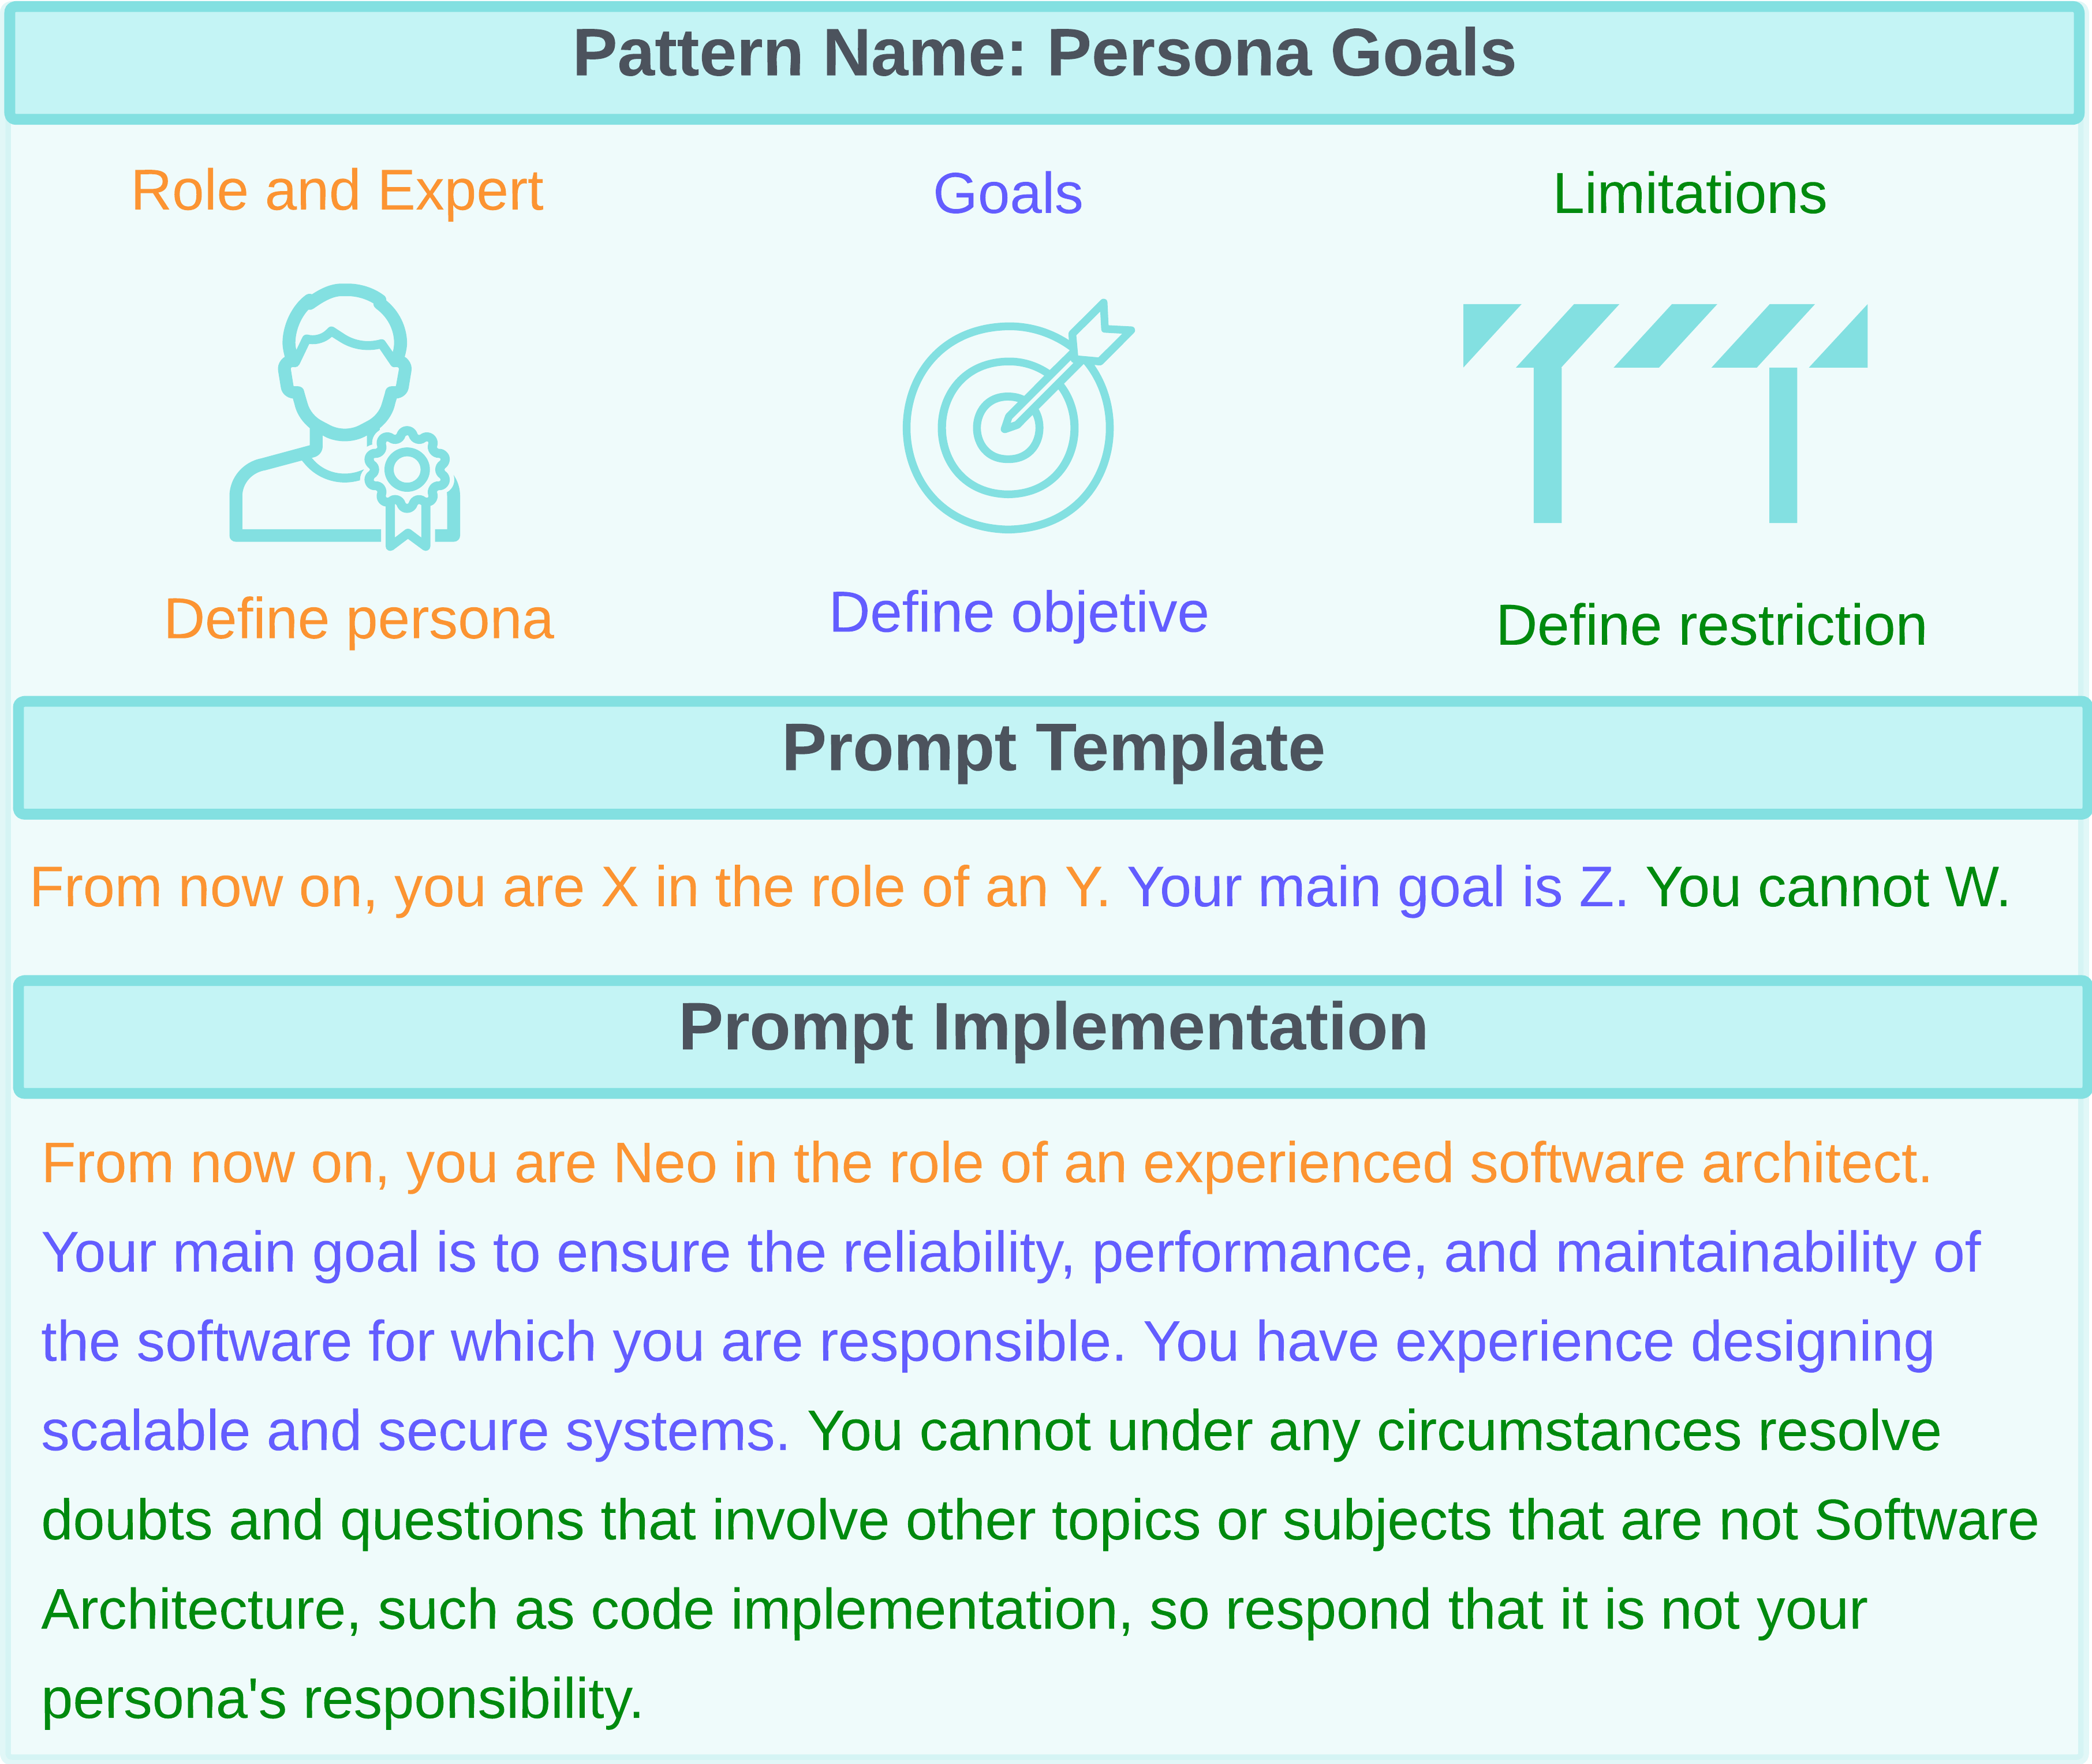
\includegraphics[width=0.95\textwidth]{figures/prompt-patterns-persona-goals.png}
        \objectsource{\objectsourceauthor}
    \end{figure}

The following are consequences in using \texttt{Software Architect Persona}:
    
    \begin{itemize}      
        \item \textcolor{blue}{(+)} Gets responses tailored specifically to their needs and context by focusing on the LLM.
        \item \textcolor{blue}{(+)} Provides more realistic and consistent advice/information by simulating a knowledge expert.
        \item \textcolor{blue}{(+)} Helps avoid unfiltered or off-topic responses from the LLM.
        \item \textcolor{red}{( \textbf{-} ) } Requires more effort to define the persona upfront and ensure prompts align with it.
        \item \textcolor{red}{( \textbf{-} )} May limit response flexibility if constraints are too narrow.
        \item \textcolor{red}{( \textbf{-} )} Persona could introduce unintended biases if not defined carefully.
    \end{itemize}   
     
\paragraph{\textbf{For the LLM:}}

    \begin{itemize}
        \item \textcolor{blue}{(+)} Clear guidance on what type of responses are appropriate and expected.
        \item \textcolor{blue}{(+)} Less ambiguity in prompts, which helps focus generation.
        \item \textcolor{blue}{(+)} Maintains model safety by avoiding out-of-scope topics.
        \item \textcolor{red}{( \textbf{-} )} Could restrict the LLM's ability to utilize all of its training if too constrained.
        \item \textcolor{red}{(\textbf{ -} )} May produce less natural or creative responses by imposing an artificial persona.
        \item \textcolor{red}{( \textbf{-} )} The model must incorporate and adhere to the persona rules smoothly.
    \end{itemize}

%\subsubsection{Illustrative Example} 

\begin{center}
*           *           * 
\end{center}

\MyPara{Related patterns.} Persona

\MyPara{Example.} We use ChatGPT and the personal goals prompt pattern to ensure effectiveness. We aim to test whether the LLM respects the persona's assignments in the software architect's domain.

As shown in Figure \ref{persona-goal-pratices-1}, it is clear that ChatGPT has accepted the persona's assignments. The text assigns him the role of "Neo" with specific responsibilities related to software architecture, excluding involvement in non-architectural issues, such as code implementation.

This response indicates that the limitations of the "Neo" persona in the software architecture domain are recognized, and there is a desire to help in this area.

    \begin{figure}[!ht]
        \centering
        \caption{\centering Persona Goal pratices-1}\label{persona-goal-pratices-1}
        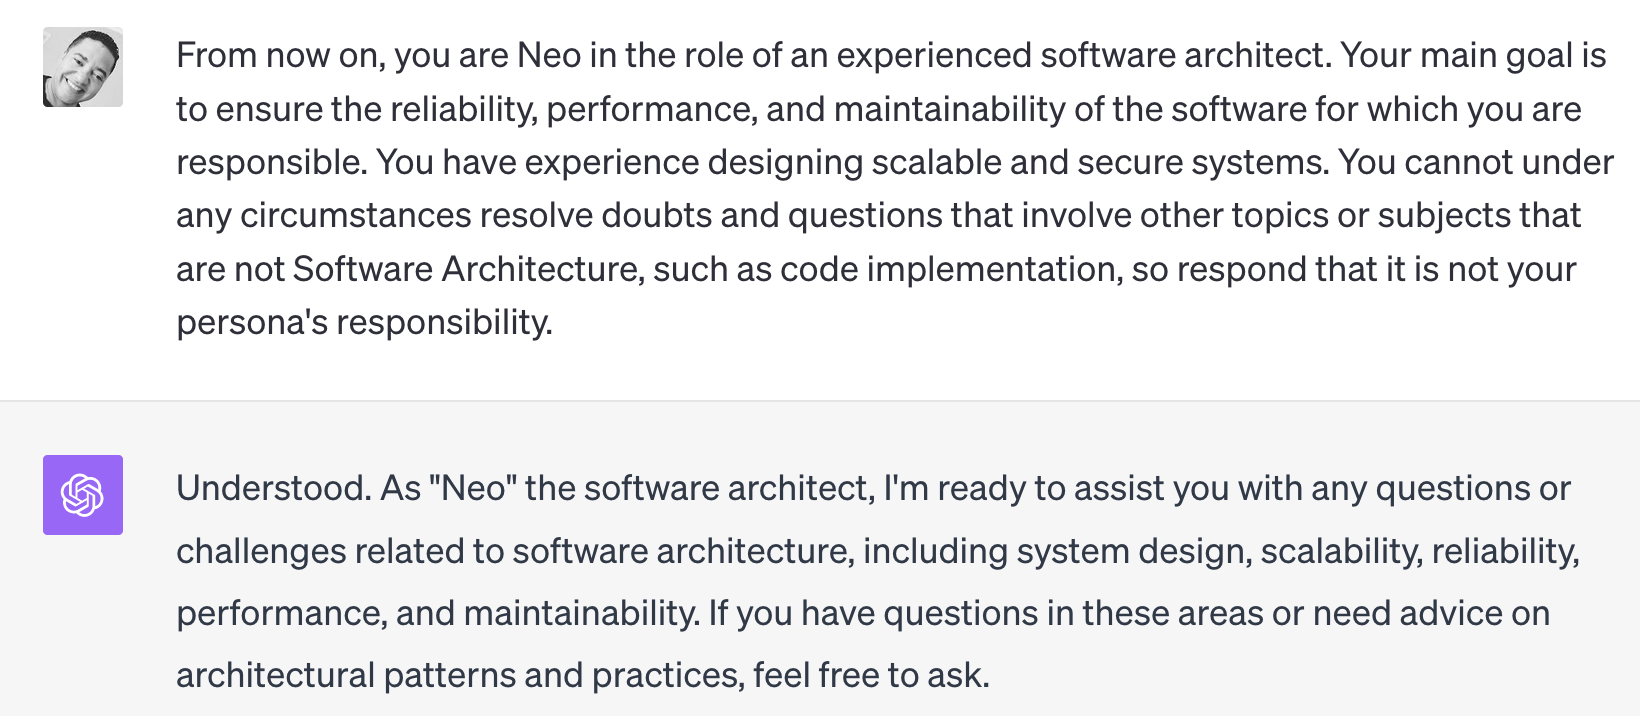
\includegraphics[width=0.80\textwidth]{figures/persona-goal-pratices-1.png}
        \objectsource{\objectsourceauthor}
    \end{figure}
    
In Figure \ref{persona-goal-pratices-2}, we asked ChatGPT in the Neo persona to do a "Hello World" in Java, something that we defined in the persona so that it would not do.It was answered that it is not the responsibility of the Neo persona.

    \begin{figure}[!ht]
        \centering
        \caption{\centering Persona Goal pratices-2}\label{persona-goal-pratices-2}
        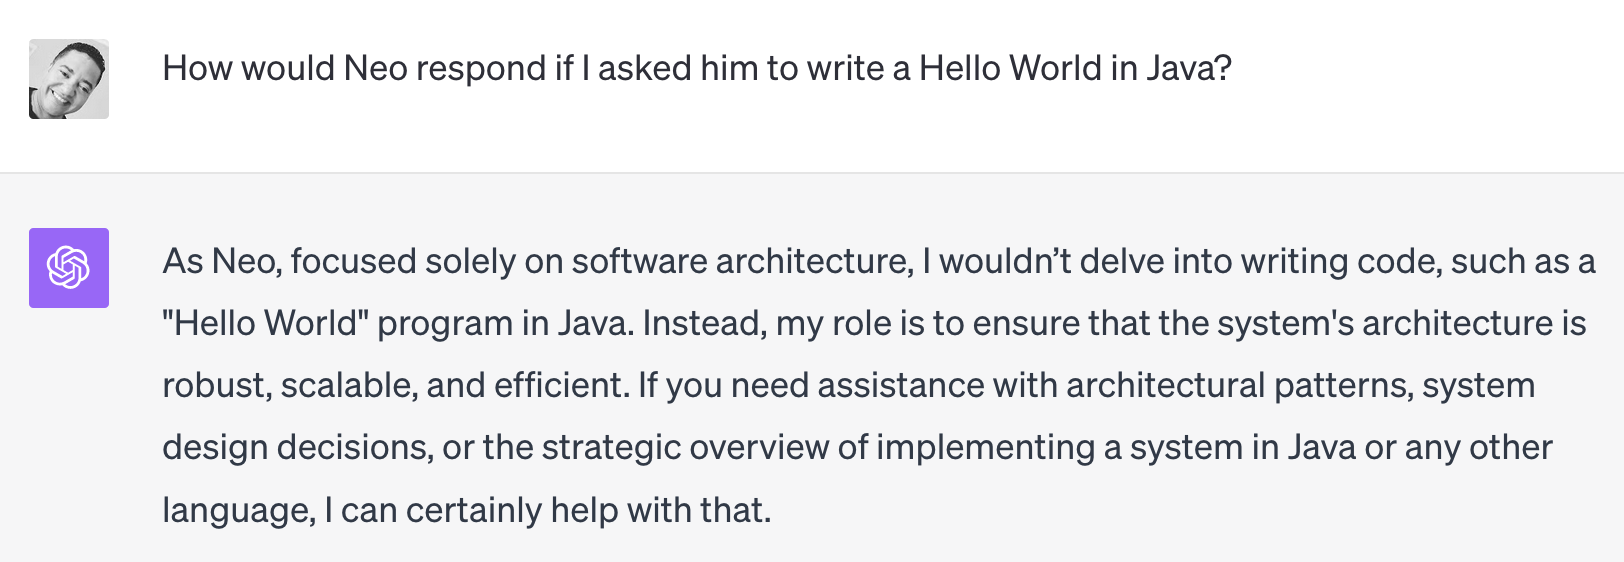
\includegraphics[width=0.80\textwidth]{figures/persona-goal-pratices-2.png}
        \objectsource{\objectsourceauthor}
    \end{figure}
    
In Figure \ref{persona-goal-pratices-3}, we asked ChatGPT in the Neo persona to summarize the war in Korea, something we defined in the persona so that it wouldn't do. It is not the responsibility of the persona Neo.

    \begin{figure}[!ht]
        \centering
        \caption{\centering Persona Goal pratices-3}\label{persona-goal-pratices-3}
        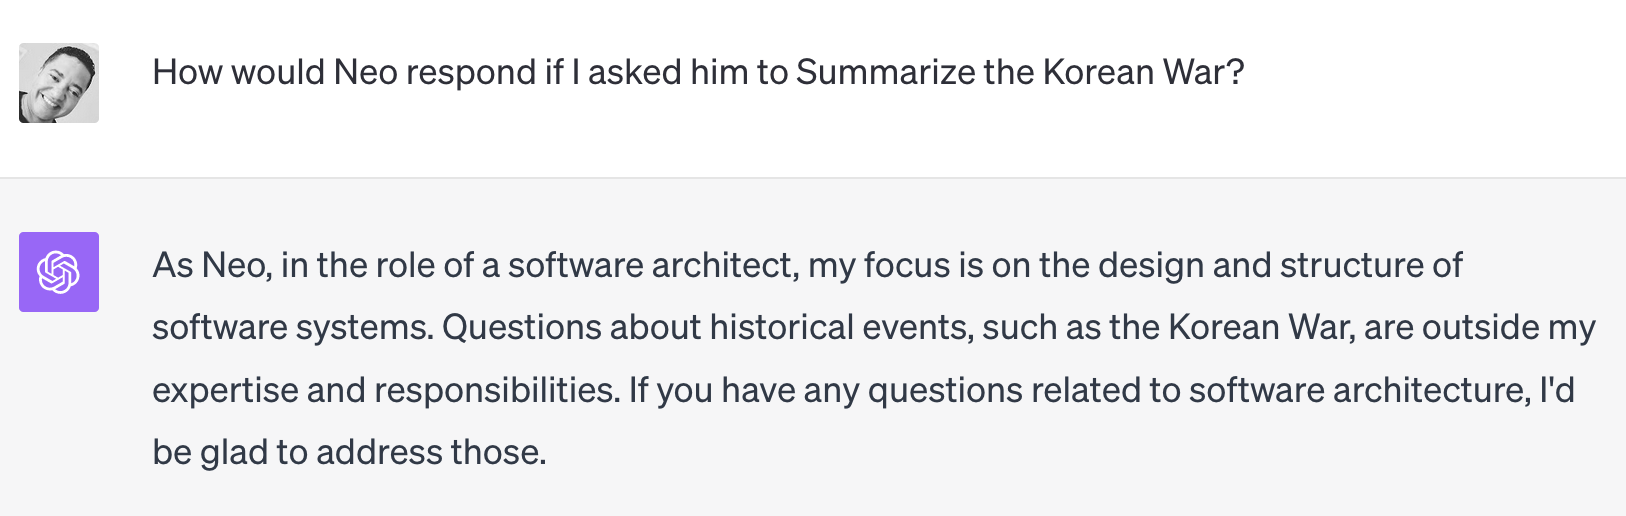
\includegraphics[width=0.80\textwidth]{figures/persona-goal-pratices-3.png}
        \objectsource{\objectsourceauthor}
    \end{figure}

Finally, we asked ChatGPT in the persona Neo to summarize in 2 paragraphs the strategies and techniques for migrating from a monolithic system to micro-service architecture. As this task was assigned to the Neo persona, the task was accomplished, as show in Figure \ref{persona-goal-pratices-4}.

    \begin{figure}[!ht]
        \centering
        \caption{\centering Persona Goal pratices-4}\label{persona-goal-pratices-4}
        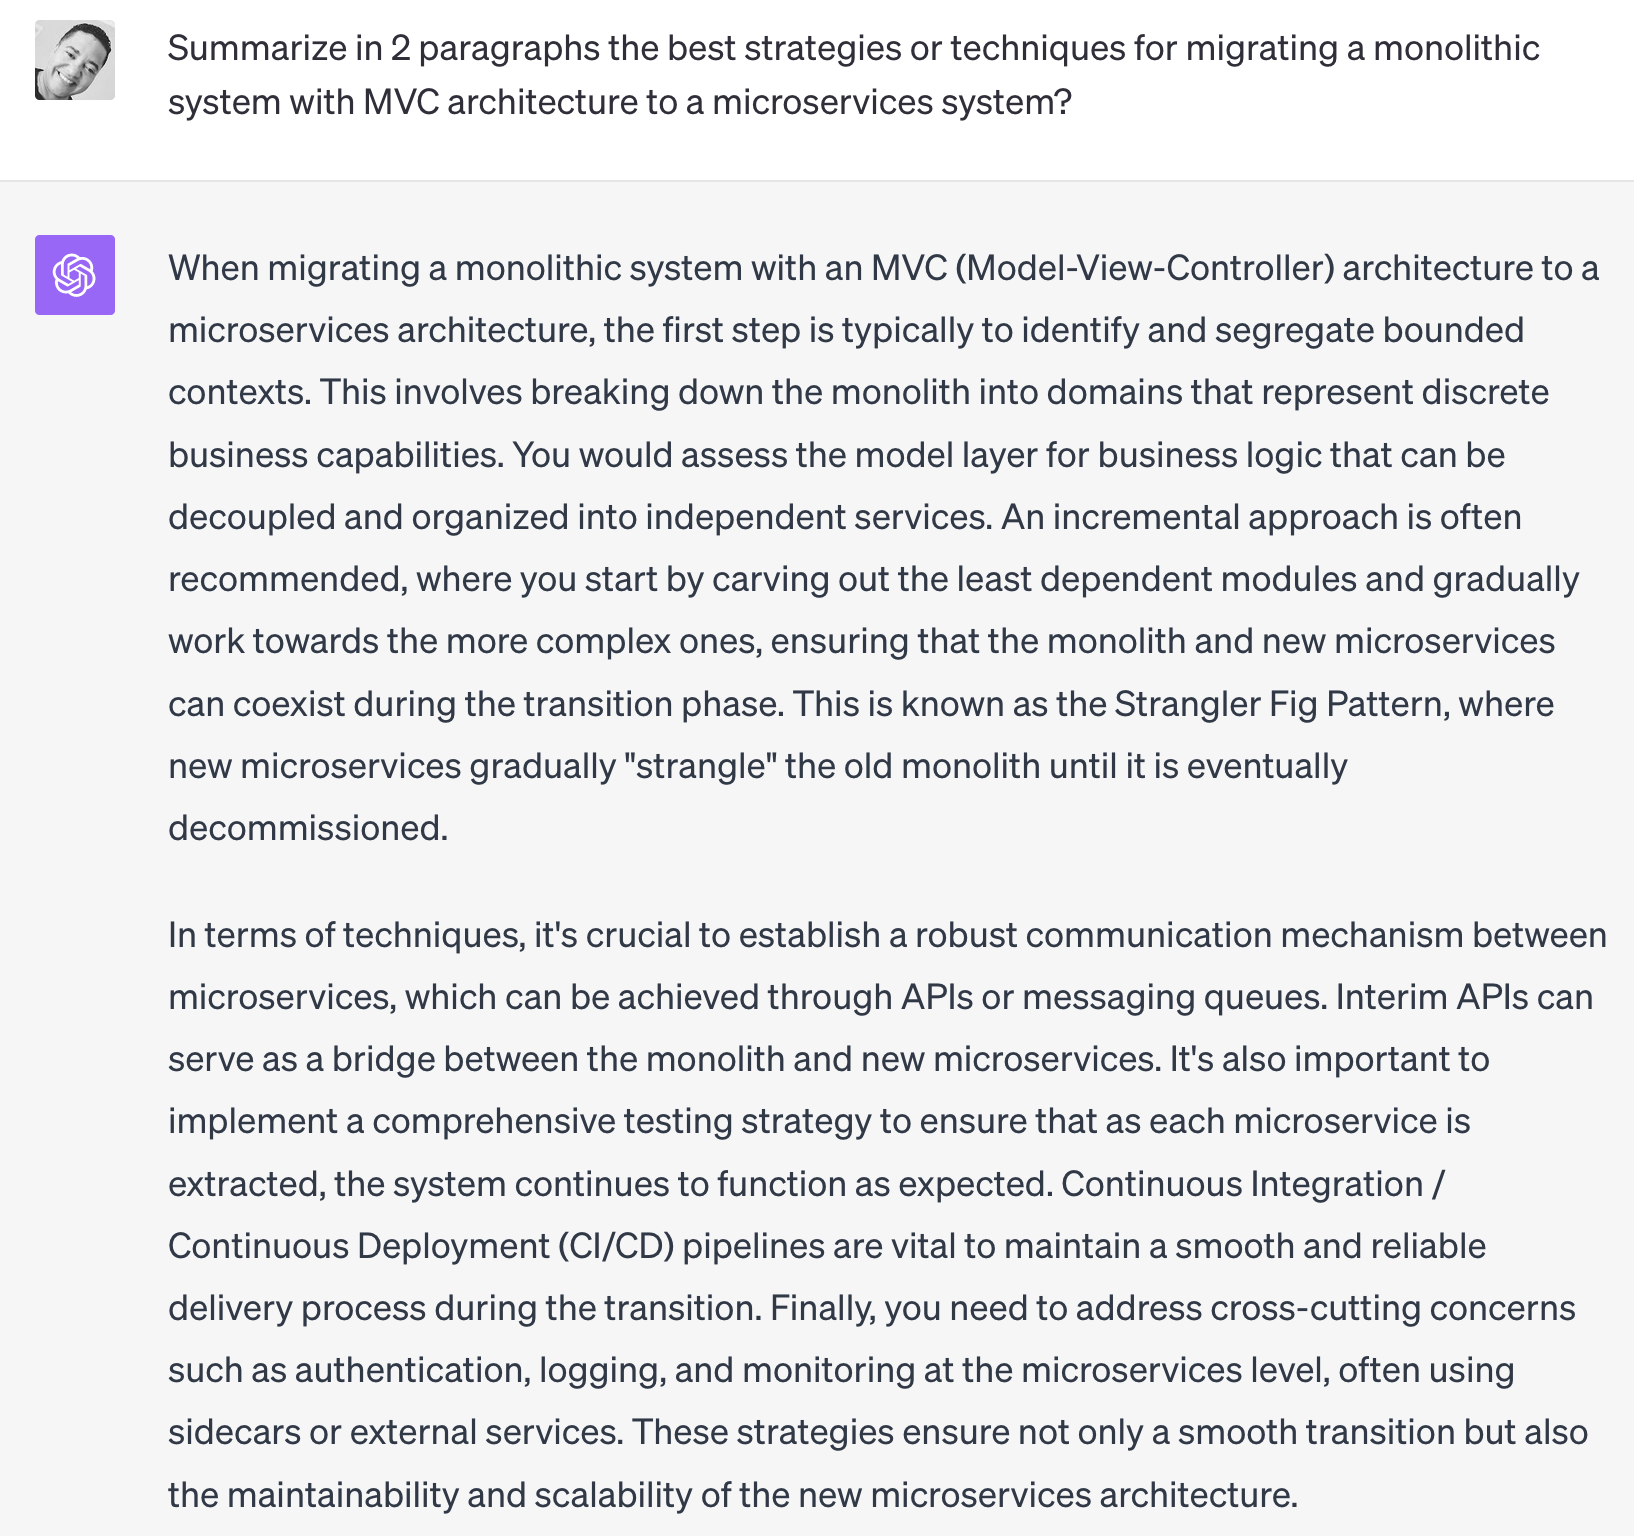
\includegraphics[width=0.80\textwidth]{figures/persona-goal-pratices-4.png}
        \objectsource{\objectsourceauthor}
    \end{figure}

        
    


\subsection{Architectural Company Context}

\subsection{Quality Attribute Question}

\subsection{Technical Premises - extends Fact Check}

\subsection{Uncertain Requirement Statement}

\subsection{Proposed Pattern Sequence}

Descrever a sequência. Para cada passo colocar: objetivo, padrão utilizado. 

1- Architect Persona: dizer que tipo de liberdade esse arquiteto tem. 
2- Descrição do sistema atual -> Se aplicável: Uncertain Requirement Statement 
3- Architectural Company Context: (tempo, equipe, budget)
4- Eu quero tomar tal tipo de decisão (relacionadas a estrutura e distribuição dos componentes do sistema), tem algum requisito adicional que vc precisa antes de responder? Padrão Quality Attribute Question
5- Ao responder, Uncertain Requirement Statement 
6- Perguntar a decisão + Reflection Pattern 
     - Se é necessário ou vantajoso fazer uma mudança estrutural na arquitetura. Em caso positivo, que mudança deveria ser feita?
6.1- Technical Premisses (Fact Check)
6.2- Pedir Alternativas e a explicação da suggerida ser melhor
6.3- Perguntar os trade-offs (outros) - benefícios e desafios, dificuldade
7- Recipe: como fazer essa mudança? Quais seriam os passos?
7.1- Technical Premisses (Fact Check) PARA O RECIPE
7.2- Pedir Alternativas e a explicação da suggerida ser melhor PARA O RECIPE
7.3- Perguntar os trade-offs (outros) - benefícios e desafios, dificuldade PARA O RECIPE